%---------------------导言区---------------------------%
\documentclass[12pt,a4paper,UTF8]{ctexart}
\usepackage{geometry}
	\geometry{left=2.5cm,right=2.5cm,top=3.2cm,bottom=2.8cm}
\usepackage{xeCJK,amsmath,paralist,enumitem,booktabs,multirow,graphicx,subfig,setspace,listings,lastpage}
	\setlength{\parindent}{2em}
	\lstset{language=Python}
\usepackage{fancyhdr}
	\pagestyle{fancy}
	\rhead{B1 光电效应实验}
	\lhead{基础物理实验\uppercase\expandafter{\romannumeral2}简要实验报告}
	\cfoot{Page \thepage/\pageref{LastPage}}  %当前页\总页数
	\rfoot{\today}
	\renewcommand{\headrulewidth}{0.4pt}
	\renewcommand{\theenumi}{(\arabic{enumi})}
\usepackage[colorlinks,linkcolor=blue,urlcolor=blue,citecolor=blue]{hyperref}
%%%%%%%%%%%%%%%%%%%%%%%%%%%%%%%%%%%%%%%%%%%%%%%%%%%%%%%%%%
%%%%%%%%%%%%%%%%%%%%%%%%%正文开始%%%%%%%%%%%%%%%%%%%%%%%%%%
%%%%%%%%%%%%%%%%%%%%%%%%%%%%%%%%%%%%%%%%%%%%%%%%%%%%%%%%%%

\begin{document}

%%begin-------------------标题与信息-----------------------%%
%%标题
\begin{center}
\LARGE\textbf{B1 光电效应实验}
\end{center}

%%信息
\begin{doublespacing}
	\centering
	\begin{tabular}{ll}
	 & \\
	{\CJKfontspec{Droid Sans Fallback} 实验人:黄子维 20980066} & {\CJKfontspec{Droid Sans Fallback}合作者:黄睿杰 20980062}\\
	{\CJKfontspec{Droid Sans Fallback} 实验时间:2021.12.9~星期四~上午} & {\CJKfontspec{Droid Sans Fallback} 室温:21$^{\circ}$C~相对湿度:47\%}
	\end{tabular}
\end{doublespacing}
%%end-------------------标题与信息-----------------------%%

\subsection*{【数据处理及分析】}
	\subsubsection*{1. 零电流法测量普朗克常量$h$}
		\paragraph{实验结果}~
        \newline
		\indent
        光源与光电管距离$40cm$,取口径$\phi 4mm$光阑,安装不同波长的滤光片,测量光电流为零时的反向电压值。
        结果如表\ref{tab:1},图\ref{fig:1}。
        \begin{table}[htbp]
            \centering
                \begin{tabular}{cccc}
                    \toprule
                    波长$\lambda /nm$	&频率$\nu/10^{14}s^{-1}$    &$I_{U_{AK}=2V}/10^{-13}A$   &截止电压$U_0 /V$  \\
                    \midrule
                    365    &8.22    &-20	&1.782    \\
                    405    &7.41    &-12	&1.464    \\
                    436    &6.88    &-17	&1.240    \\
                    546    &5.49    &-5    	&0.715    \\
                    577    &5.20    &-2 	&0.612    \\
                    \bottomrule
                \end{tabular}
                \caption{\textbf{各谱线对应截止电压}}
                \label{tab:1}
        \end{table}

		\begin{figure}[htbp]
			\centering
			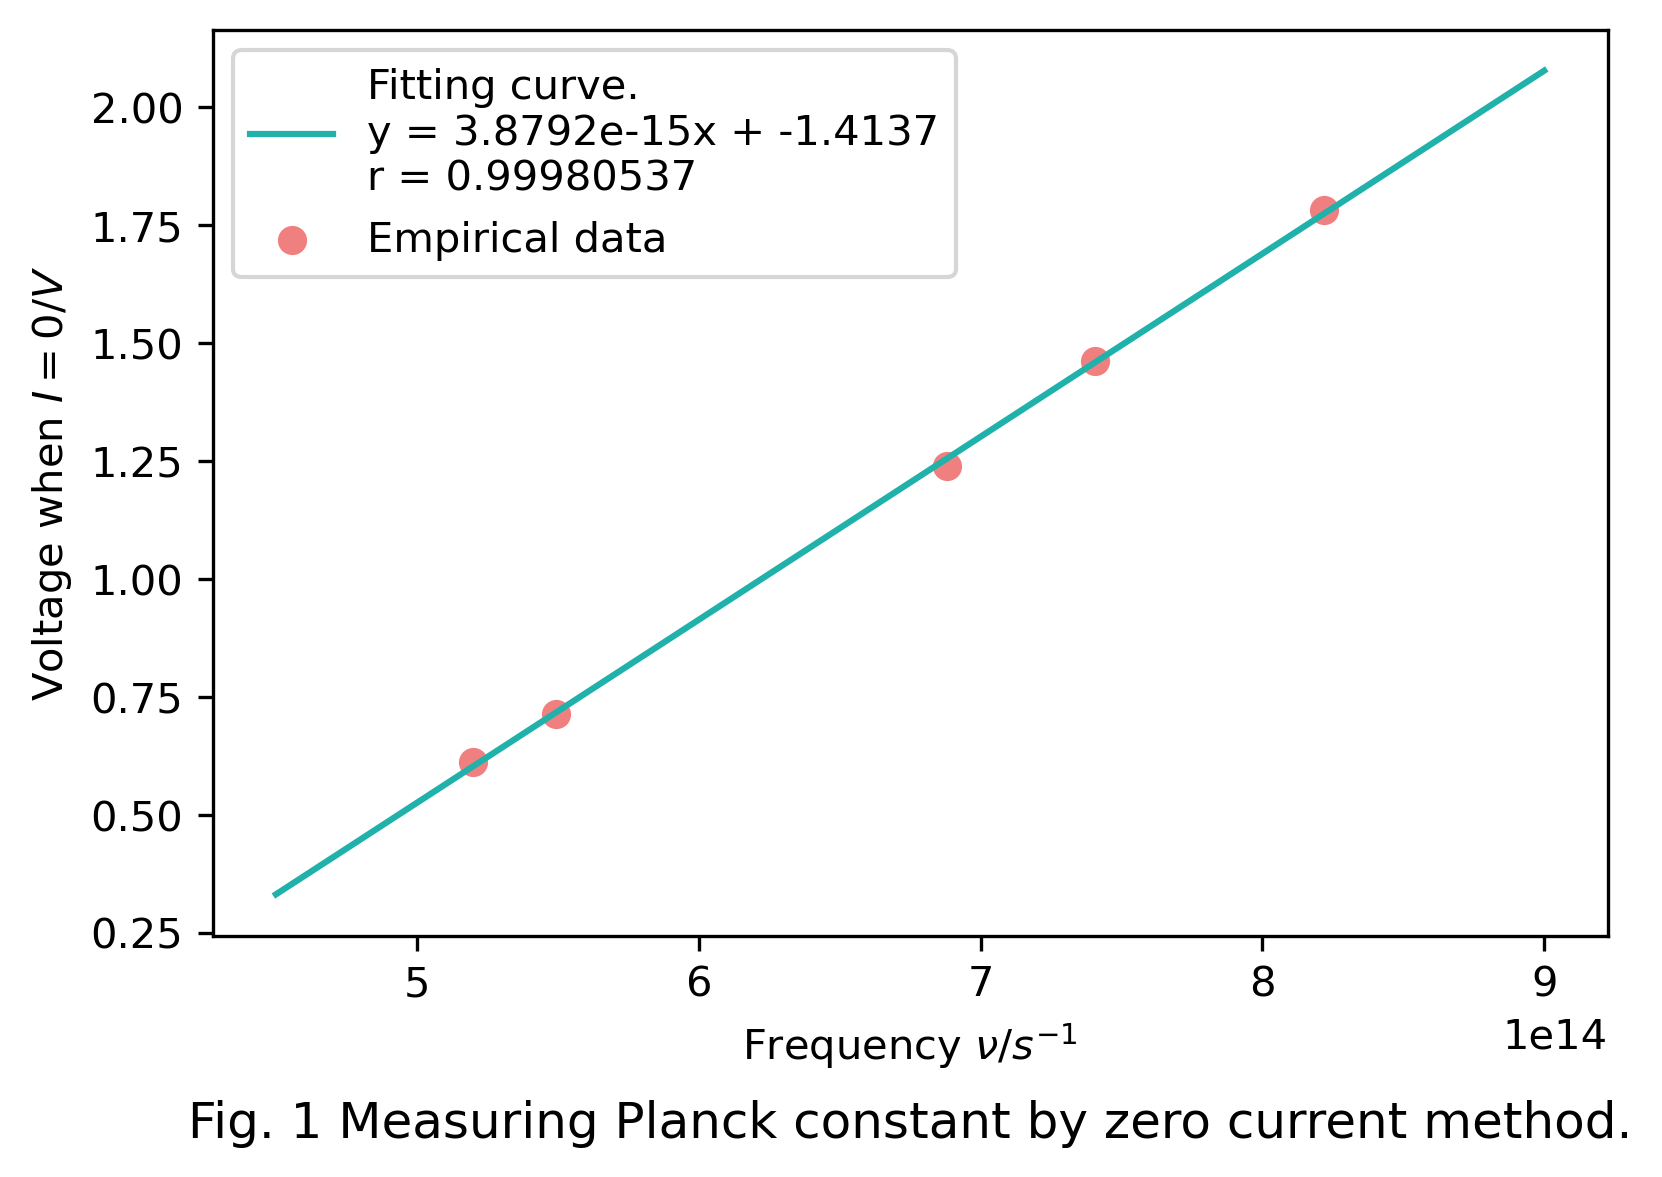
\includegraphics[width=0.7\textwidth]{attachments/fig.1.png}
			\caption{截止电压和谱线对应频率关系}
			\label{fig:1}
		\end{figure}
        \paragraph{计算普朗克常量}~
        \newline
		\indent
        采用最小二乘法拟合图线,相关系数$R>0.99$,拟合效果好。计算拟合系数得斜率
        $$
            K = 3.88 \times 10^{-15}       
        $$
        由爱因斯坦光电效应理论,普朗克常量$h = Ke$,代入斜率和元电荷($e = 1.60 \times 10^{-19} C$)计算得
        $$
        h = Ke = 6.21 \times 10^{-34} J \cdot s
        $$
        对比公认值$h_0 = 6.6 \times 10^{-34} J \cdot s$,相对误差为$6.35\%$。
        
        
    \subsubsection*{2. 测量伏安特性曲线}
    \paragraph{$d=40cm, D=4mm$,不同入射波长}~
    \newline
    \indent
    控制$d=40cm, D=4mm$,取波长分别为$436nm, 546nm, 577nm$,结果如\ref{fig:2.1}
    \begin{figure}[htbp]
        \centering
        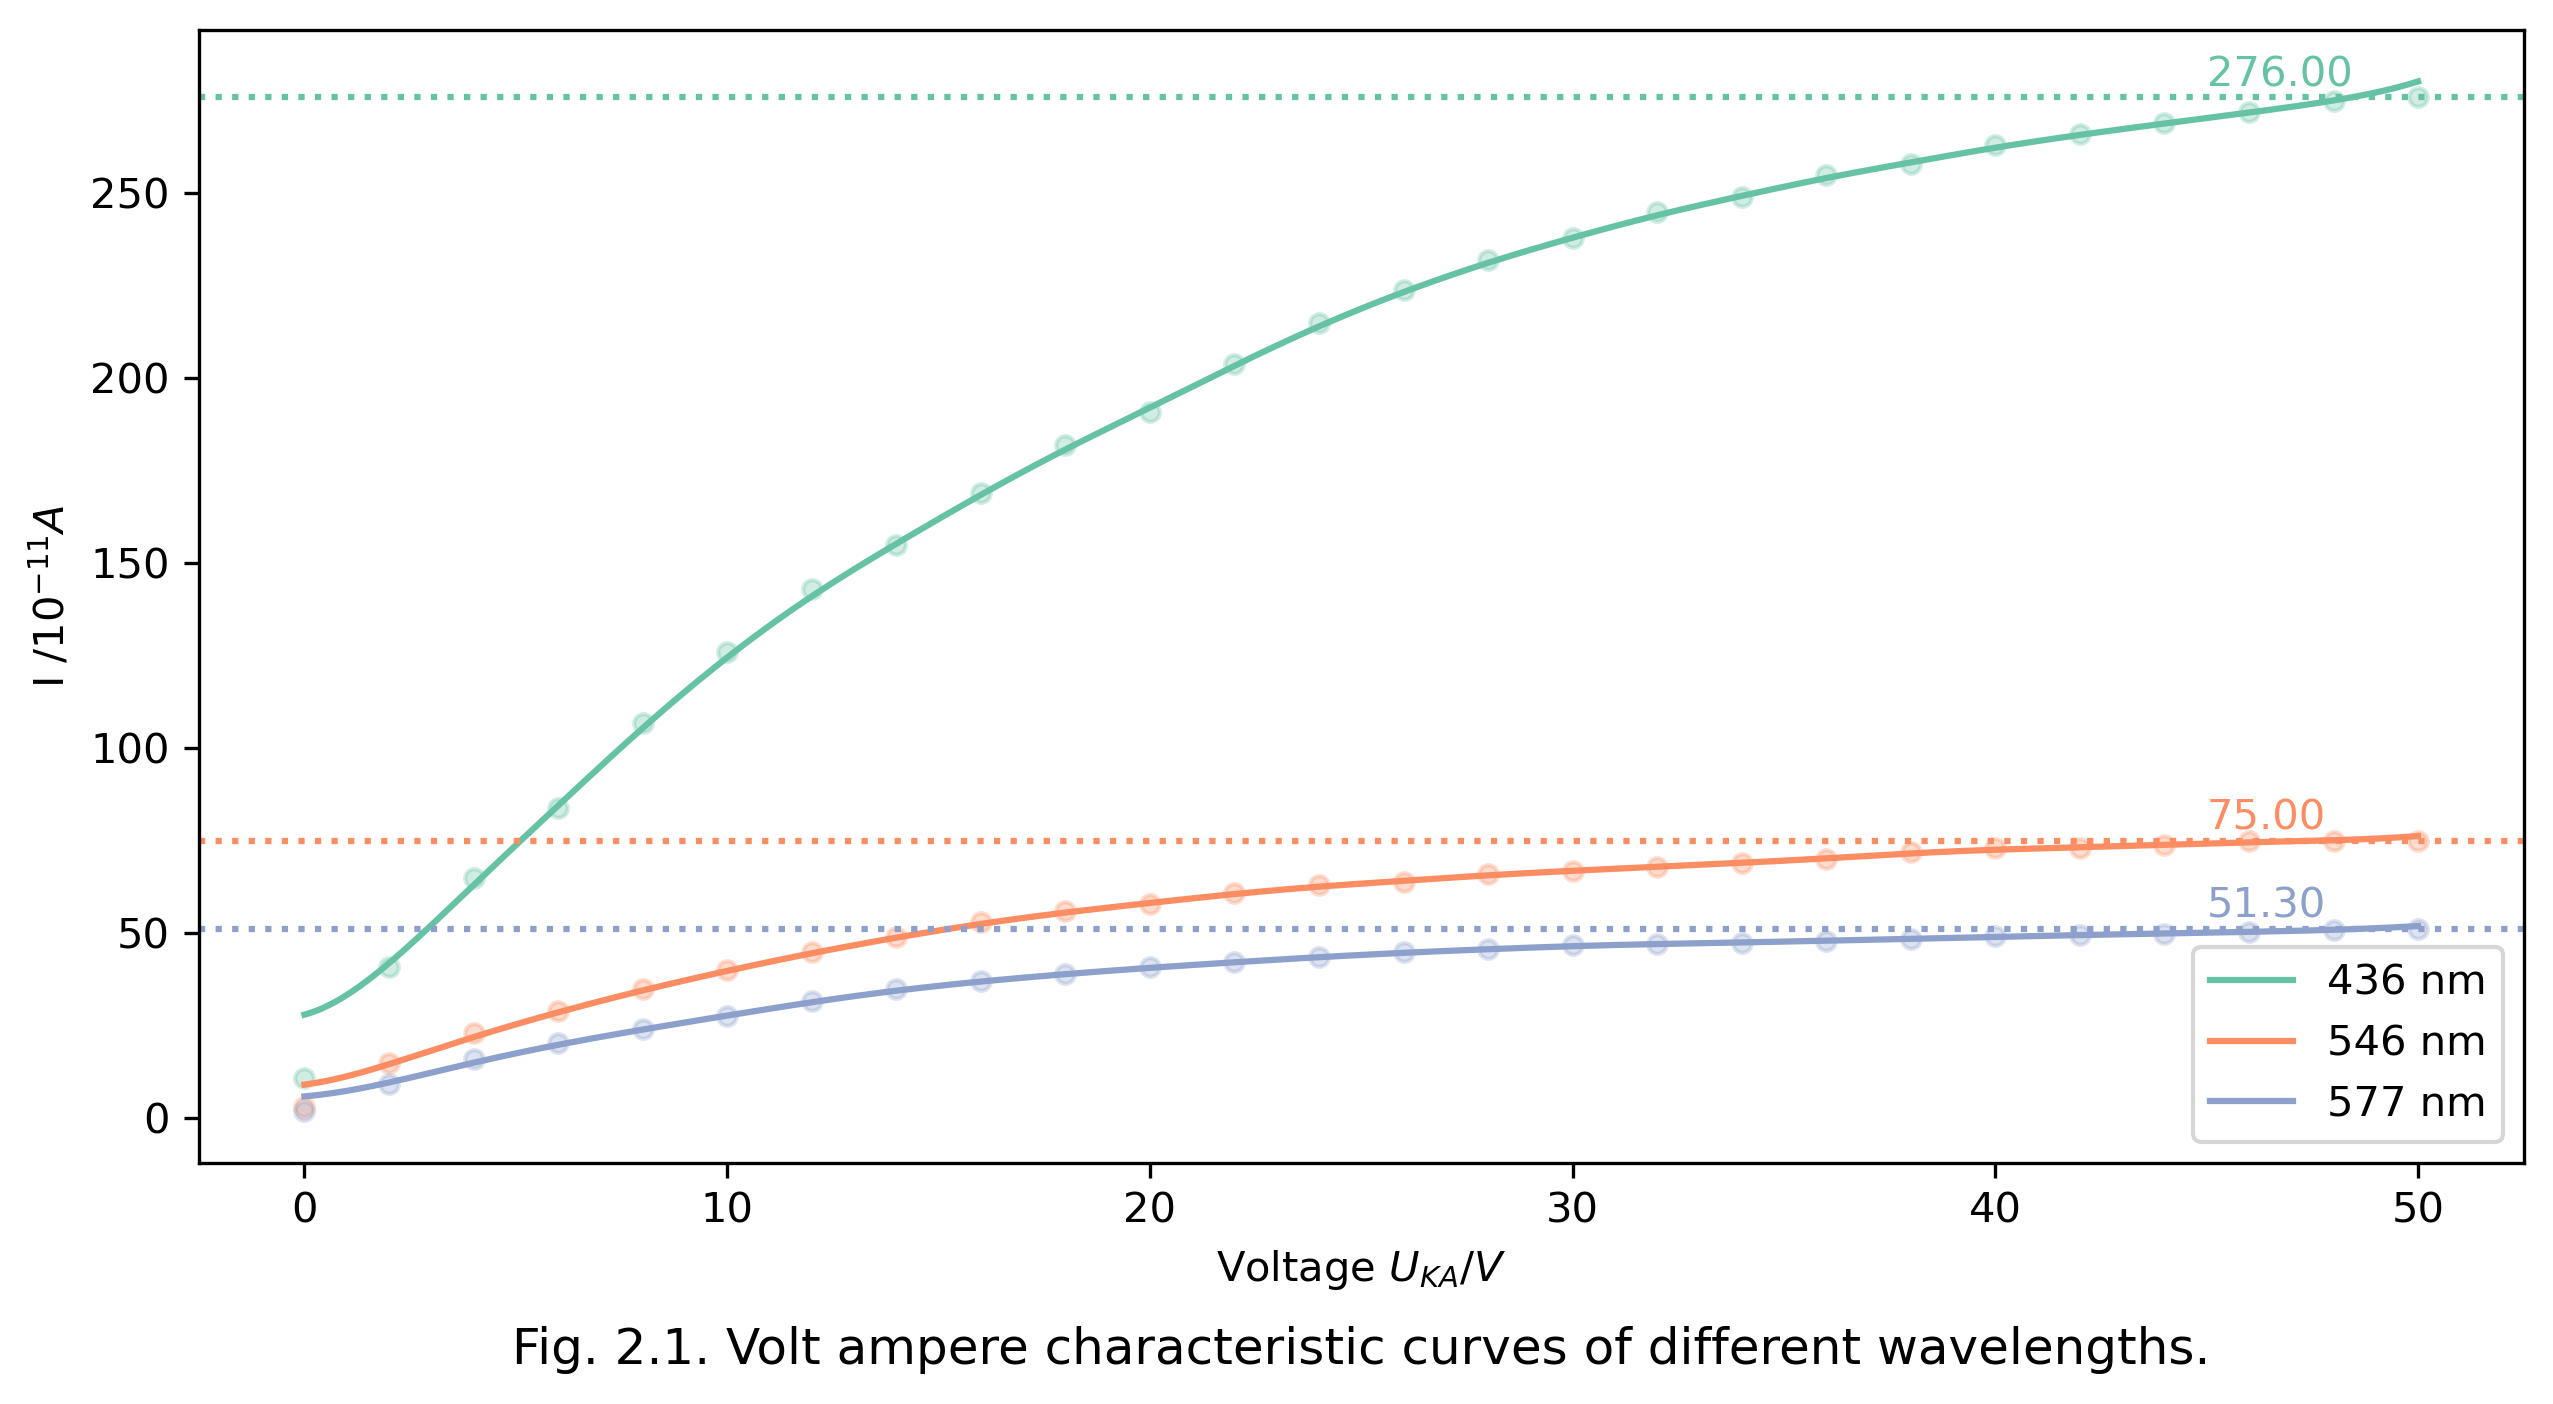
\includegraphics[width=0.7\textwidth]{attachments/fig.2.1.png}
        \caption{不同入射波长的伏安特性曲线}
        \label{fig:2.1}
    \end{figure}
    实验结果验证了当电压升高时,伏安特性曲线逐渐变缓,光电流趋于饱和。
    取$U_{AK} = 50V$时光电流作为饱和光电流,数值已在图上注明。
    随着光波长变大,饱和光电流减小。
    
    \paragraph{$\lambda=436nm, D=4mm$,不同距离}~
    \newline
    \indent
    控制$\lambda=436nm, D=4mm$,取距离分别为$40cm, 35cm, 30cm$,结果如\ref{fig:2.2}
    \begin{figure}[htbp]
        \centering
        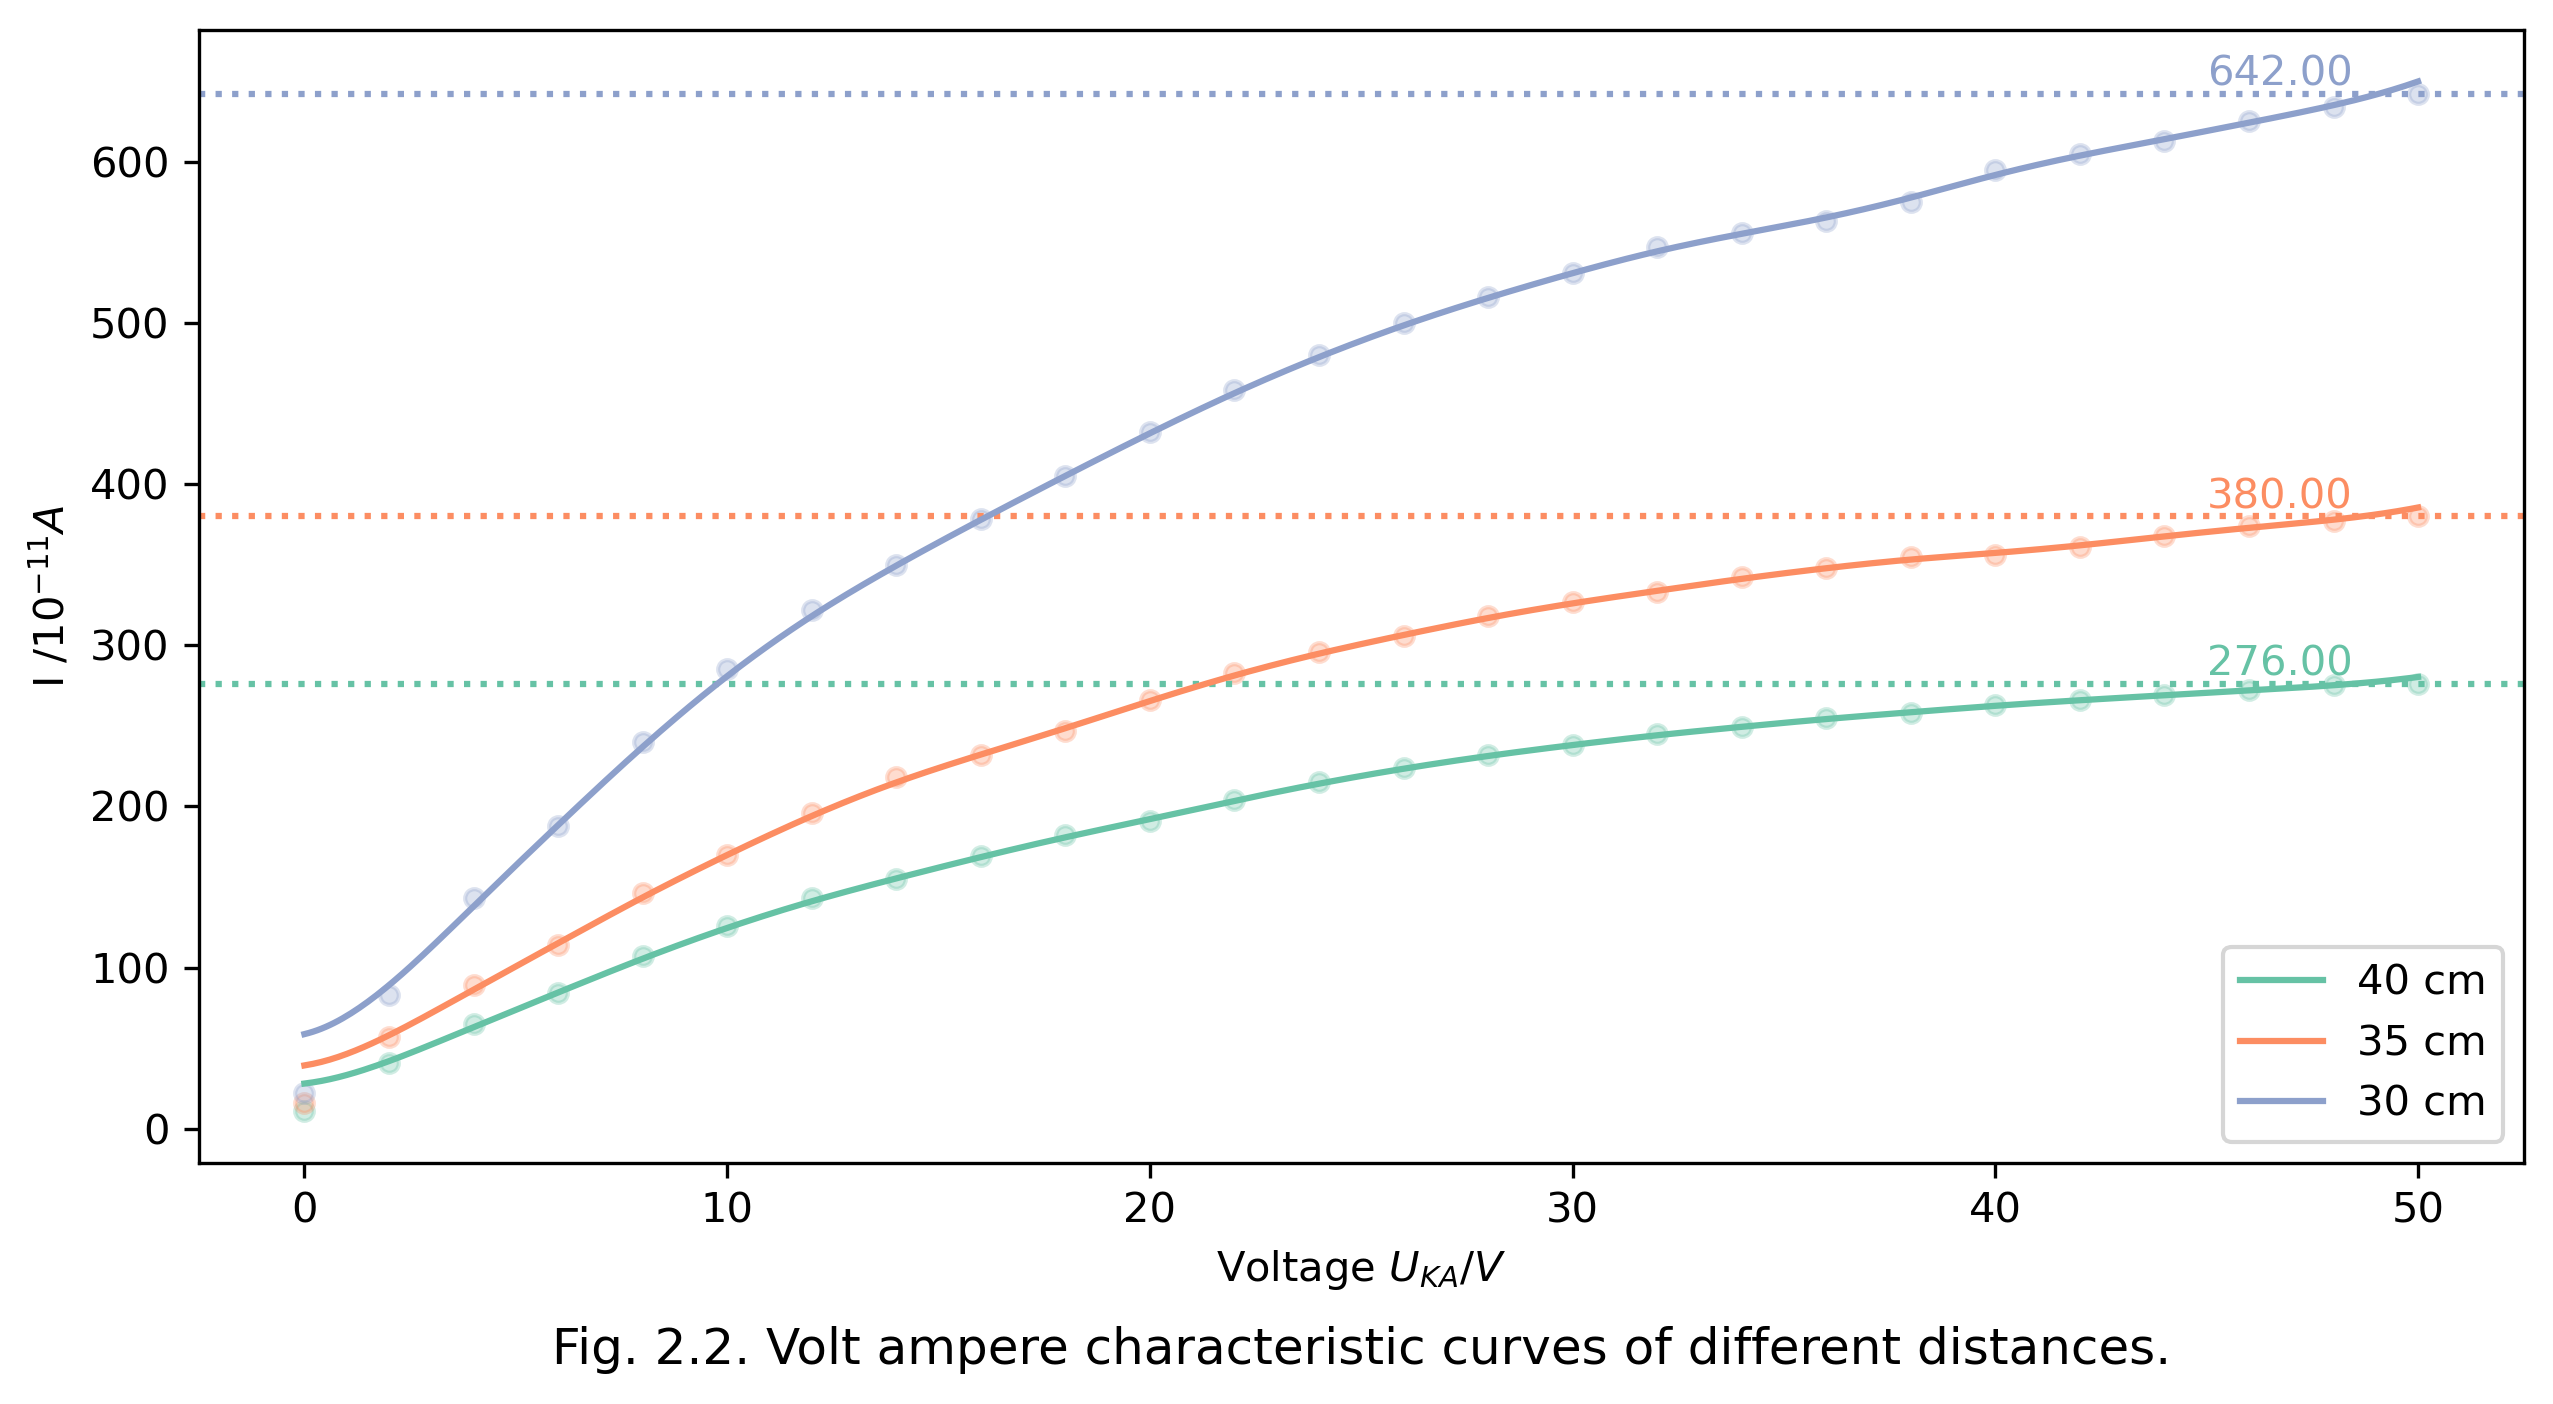
\includegraphics[width=0.7\textwidth]{attachments/fig.2.2.png}
        \caption{不同距离的伏安特性曲线}
        \label{fig:2.2}
    \end{figure}
    实验结果验证了当电压升高时,伏安特性曲线逐渐变缓,光电流趋于饱和。
    取$U_{AK} = 50V$时光电流作为饱和光电流,数值已在图上注明。
    随着距离增大,饱和光电流减小。    
    
    \paragraph{$\lambda=436nm, d=40cm$,不同光阑}~
    \newline
    \indent
    控制$\lambda=436nm, d=40cm$,取光阑孔径分别为$2mm, 4mm, 8mm$,结果如\ref{fig:2.3}
    \begin{figure}[htbp]
        \centering
        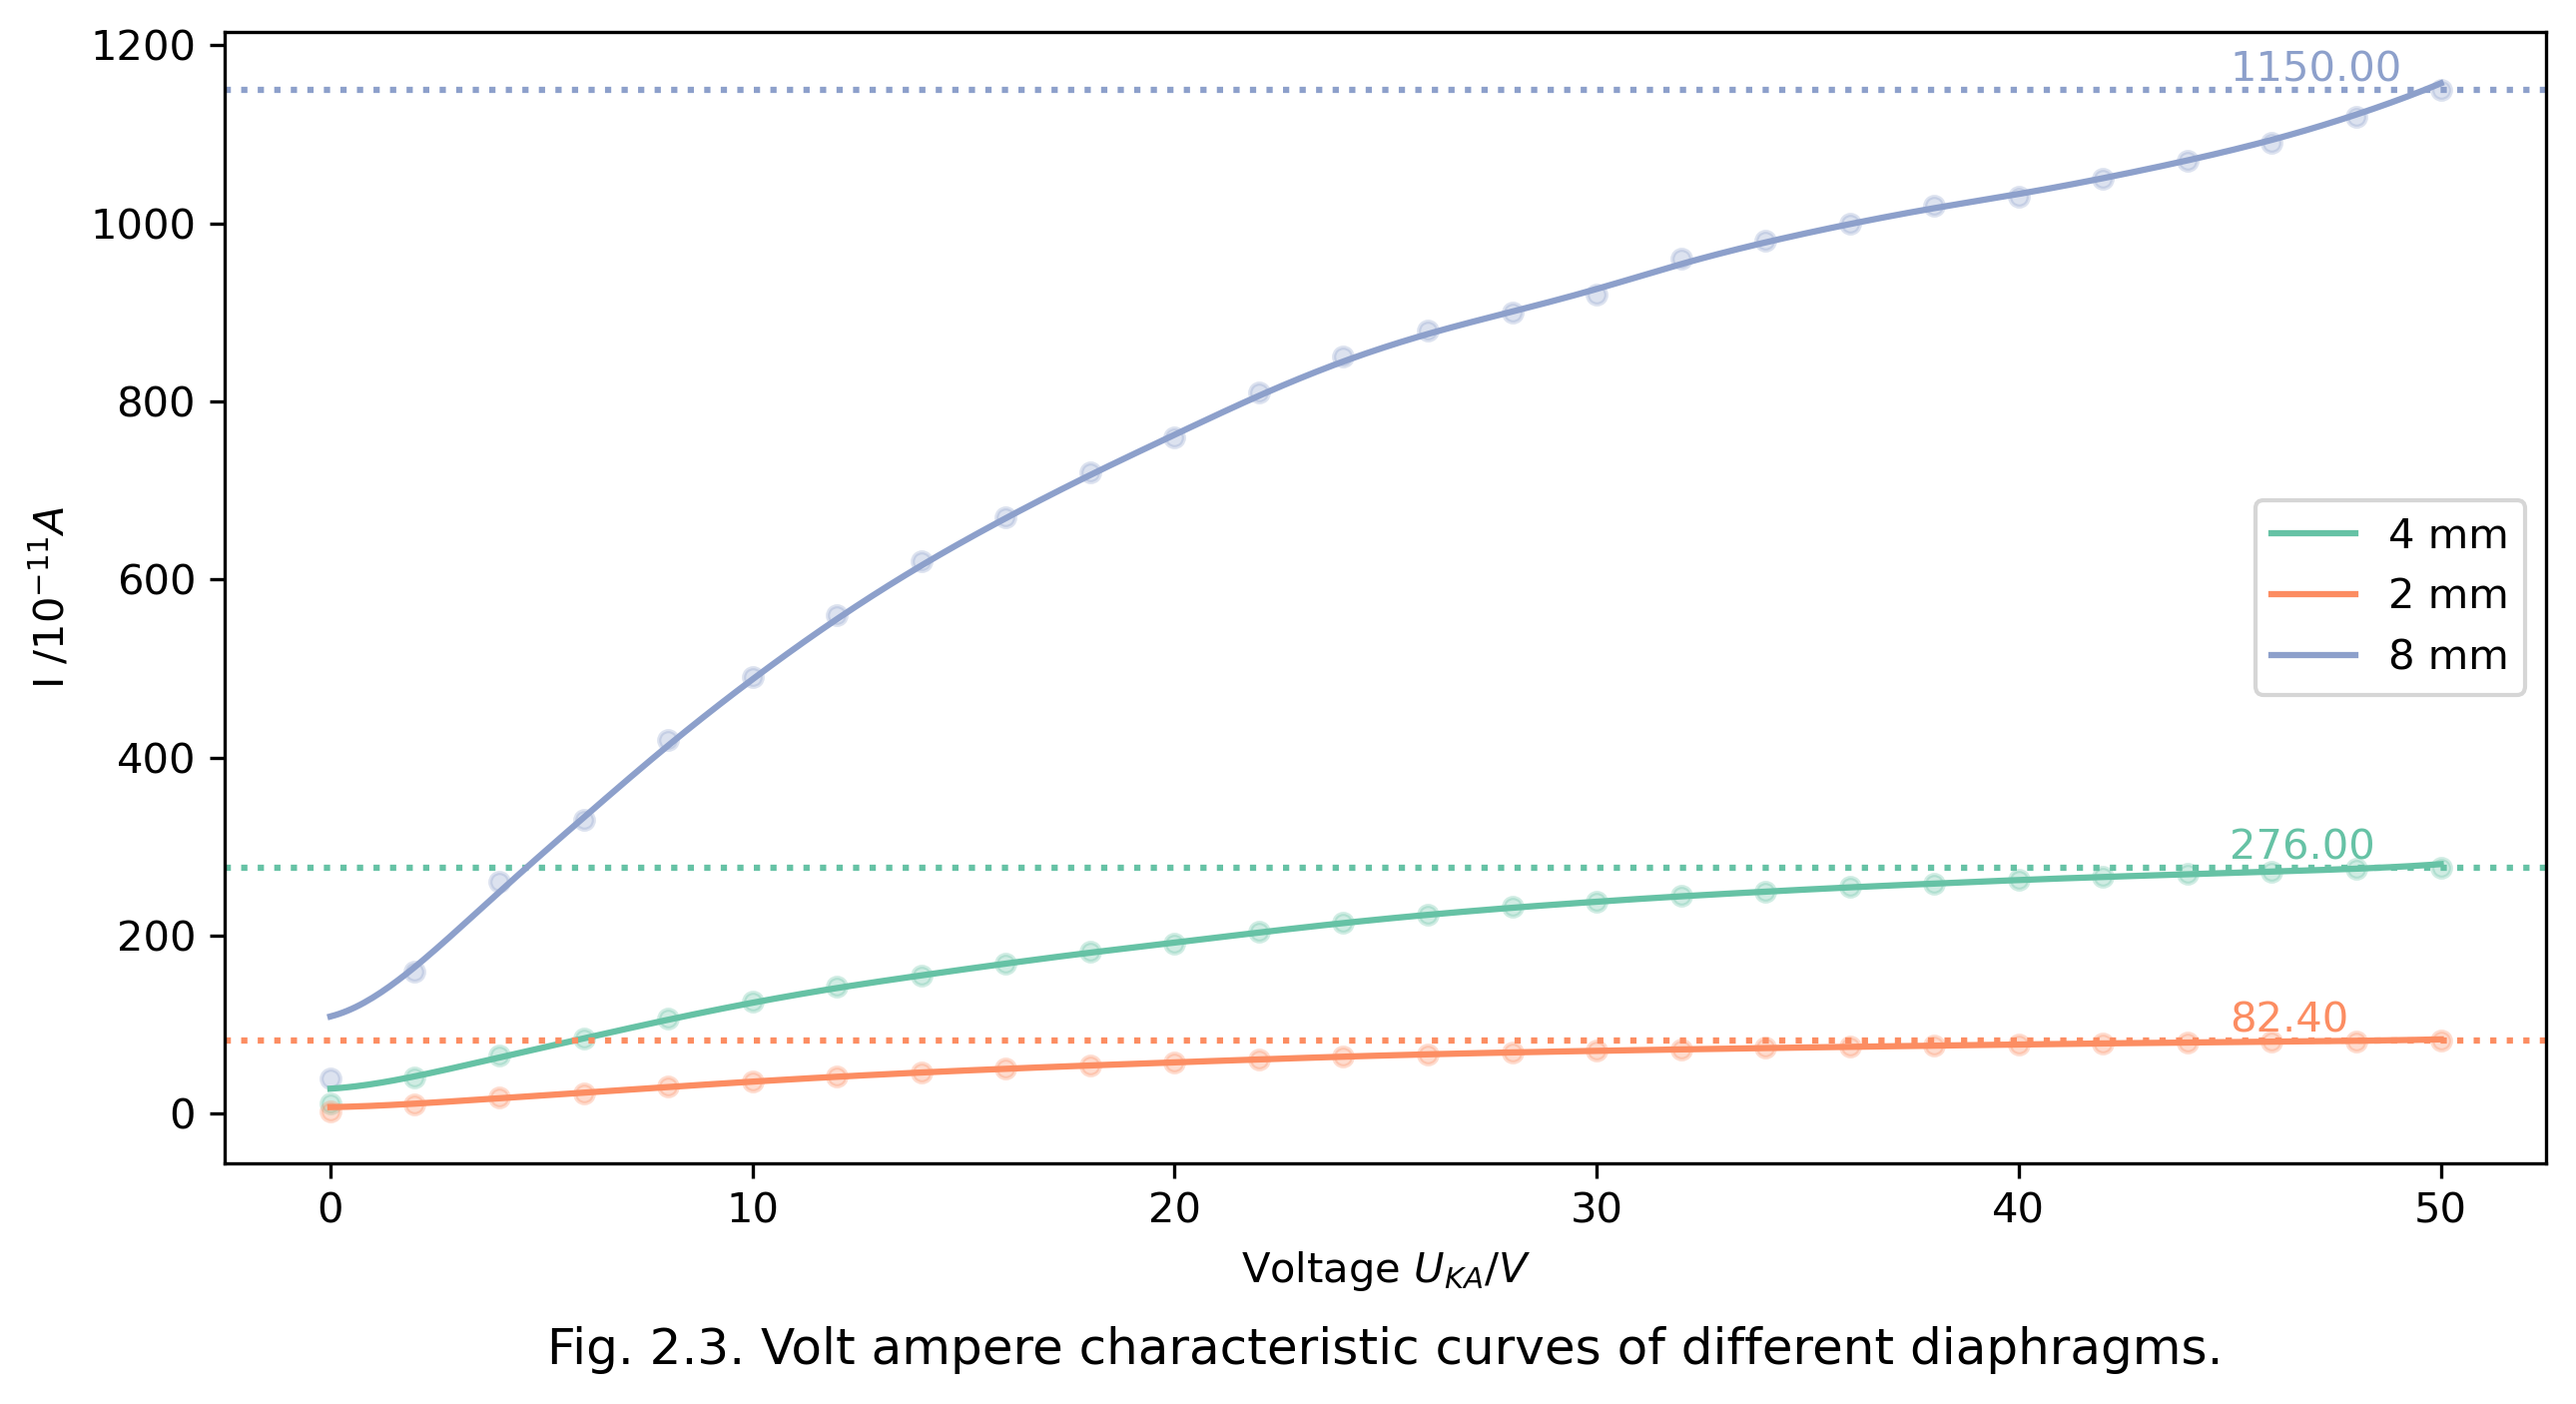
\includegraphics[width=0.7\textwidth]{attachments/fig.2.3.png}
        \caption{不同光阑的伏安特性曲线}
        \label{fig:2.3}
    \end{figure}
    实验结果验证了当电压升高时,伏安特性曲线逐渐变缓,光电流趋于饱和。
    取$U_{AK} = 50V$时光电流作为饱和光电流,数值已在图上注明。
    随着光阑口径增大,饱和光电流增大。    
    
    \subsubsection*{3. 验证饱和光电流与入射光强成正比}
    设定正向电压$U_{AK} = 50V$,分别控制光阑大小和光源距离,以探究饱和光电流和入射光强的关系。
    
    \paragraph{控制距离$d=40cm$,调节光阑大小}~
    \newline
    \indent
    结果如表\ref{tab:3.1},图\ref{fig:3.1}。
    \begin{table}[htbp]
        \centering
            \begin{tabular}{ccccc}
                \toprule
                光阑孔径$D /mm$	&光阑面积$S /mm^2$   &$I_{436nm}/10^{-11}A$   &I_{$546nm}/10^{-11}A$    &I_{$517nm}/10^{-11}A$  \\
                \midrule
                2    &3.14     &89	 &22     &14   \\
                4    &12.56    &310	 &84     &53   \\
                8    &50.26    &1180 &310    &200  \\
                \bottomrule
            \end{tabular}
            \caption{\textbf{饱和光电流和光阑面积的关系}}
            \label{tab:3.1}
    \end{table}

    \begin{figure}[htbp]
        \centering
        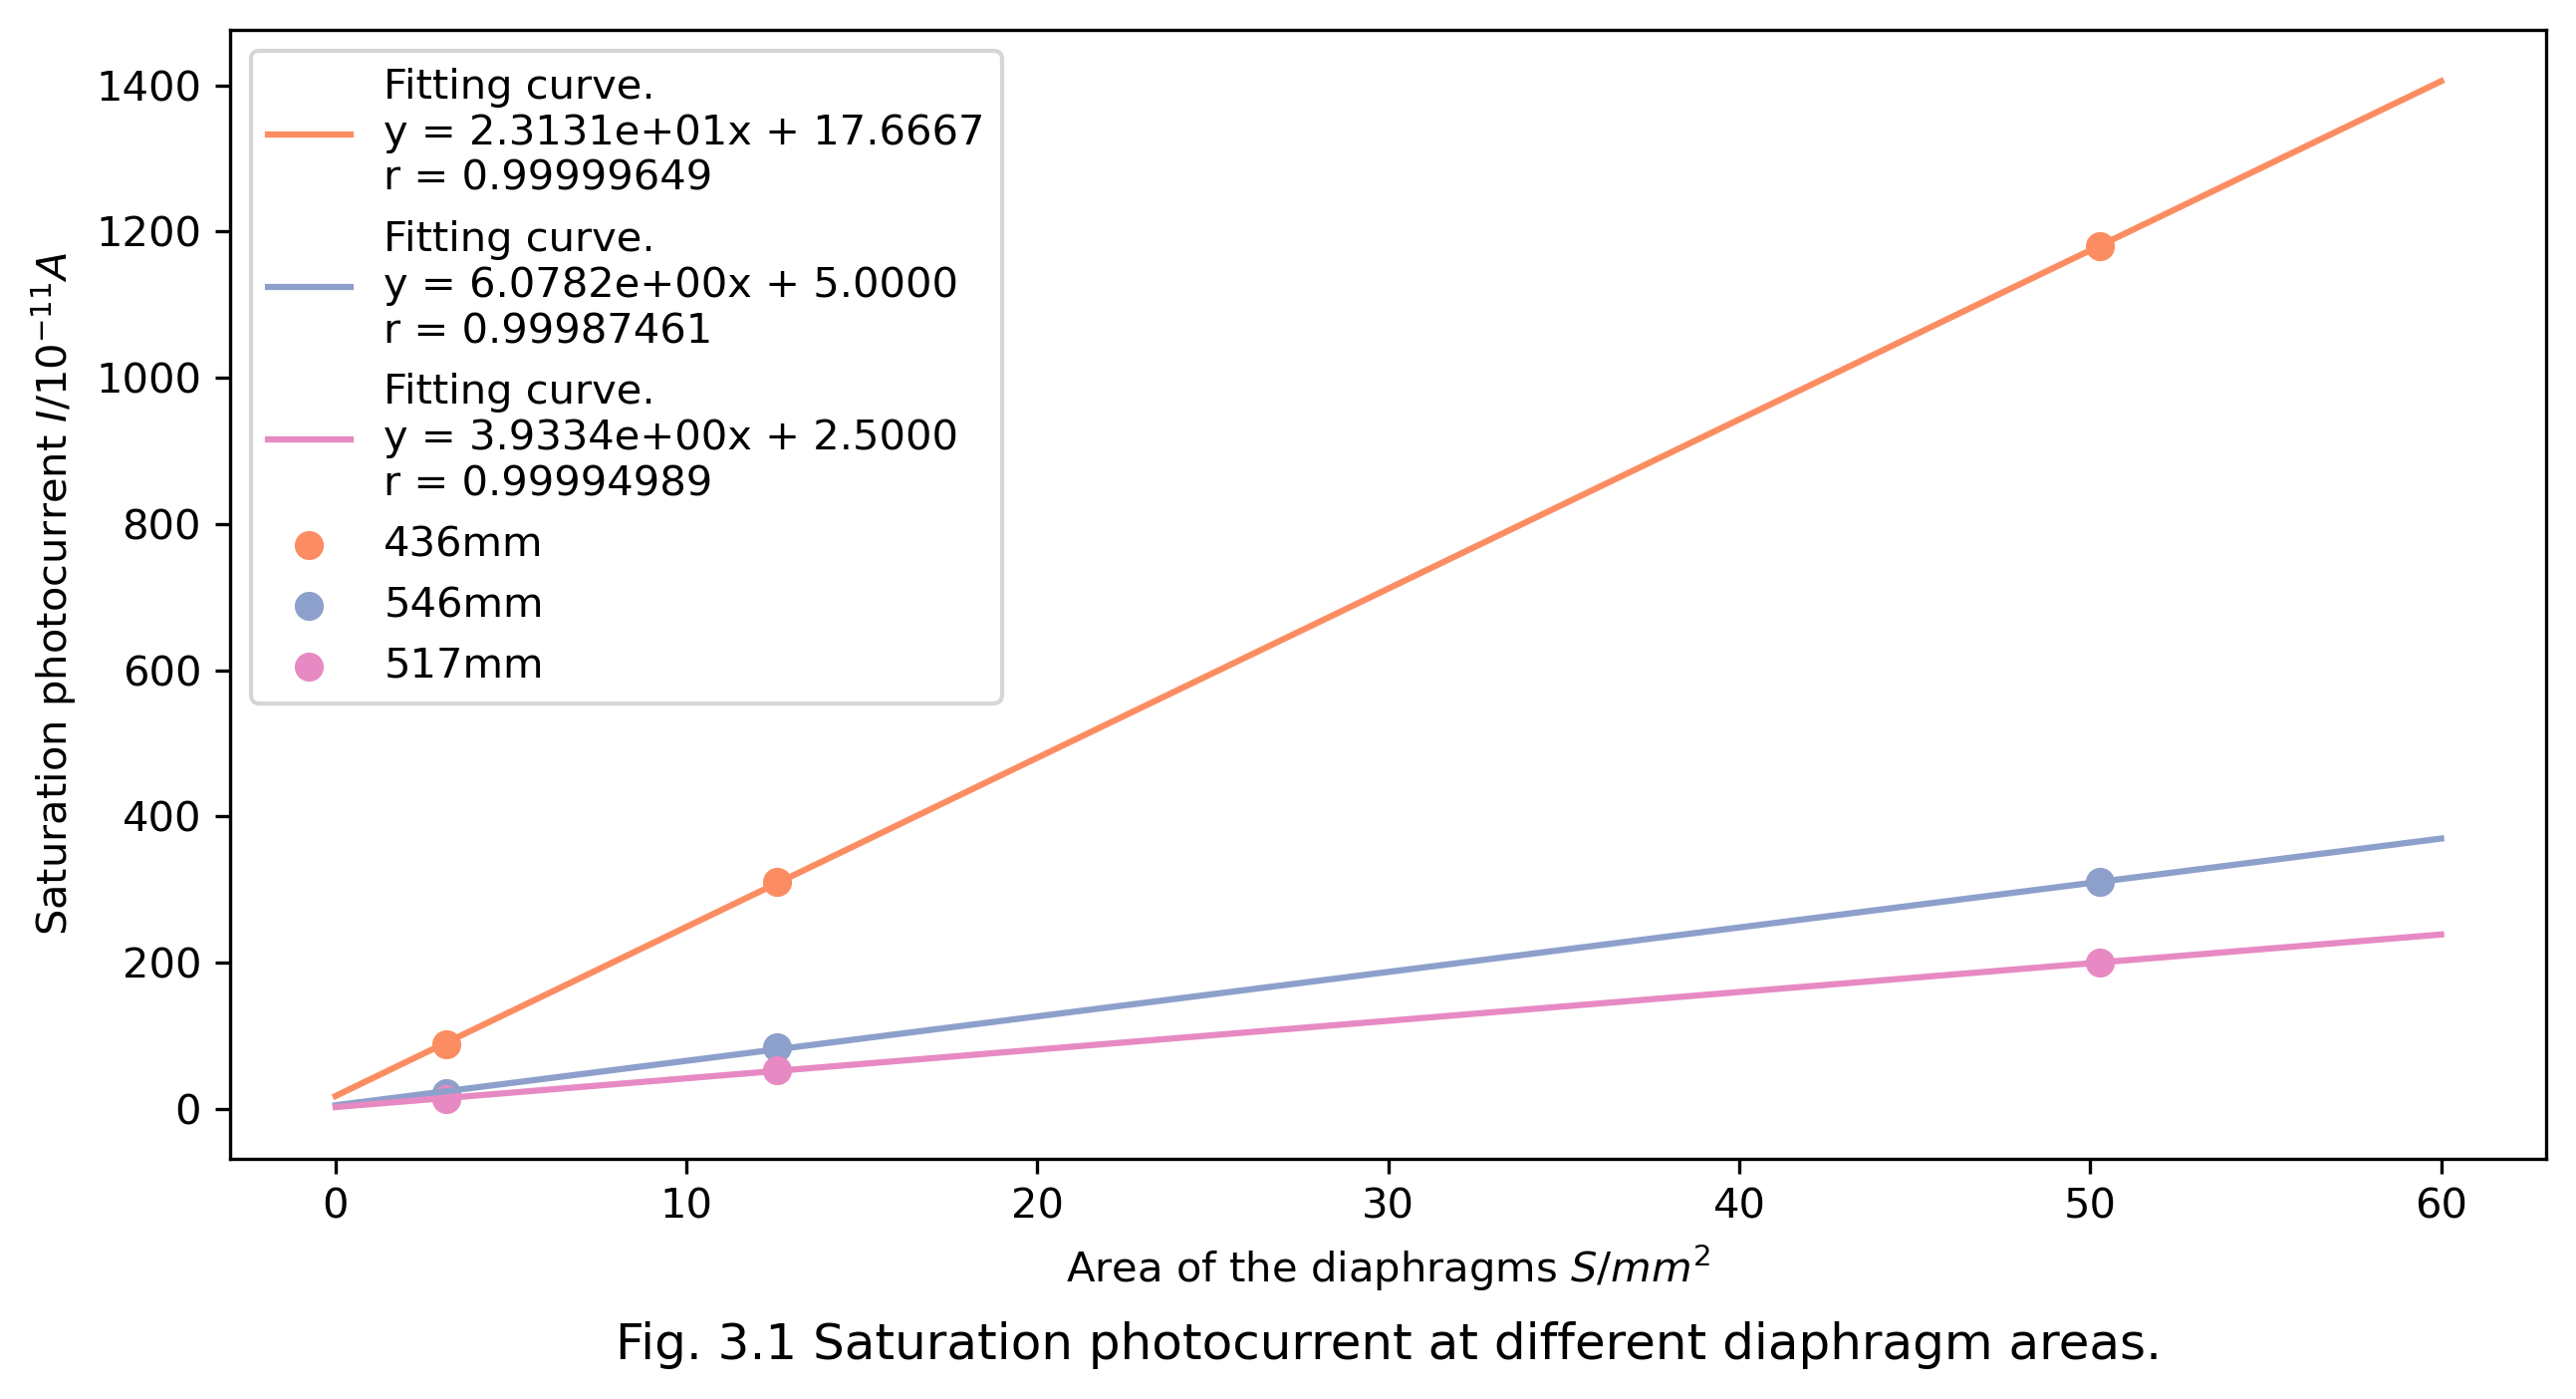
\includegraphics[width=0.7\textwidth]{attachments/fig.3.1.png}
        \caption{饱和光电流和光阑面积的关系}
        \label{fig:3.1}
    \end{figure}
    实验结果显示饱和光电流和光阑面积成线性正相关,相关系数$R>0.99$。
    而光强与光阑面积成正比,因此证明了饱和光电流与入射光强成正比。
    同时随着波长减小,饱和光电流随入射光强增长越快。

    \paragraph{控制光阑$D=4mm$,调节距离大小}~
    \newline
    \indent
    结果如表\ref{tab:3.2},图\ref{fig:3.2}。
    \begin{table}[htbp]
        \centering
            \begin{tabular}{ccccc}
                \toprule
                距离$d /cm$	&$1/d^2 /cm^{-2}$   &$I_{436nm}/10^{-11}A$   &I_{$546nm}/10^{-11}A$    &I_{$517nm}/10^{-11}A$  \\
                \midrule
                40  &0.000625   &280   &83	   &53	    \\   
                38  &0.000693   &320   &95	   &61	    \\
                36  &0.000772   &380   &110    &70	    \\
                34  &0.000865   &440   &128    &81	    \\
                32  &0.000977   &520   &150    &97	    \\
                30  &0.001111   &620   &178    &112	    \\
                \bottomrule
            \end{tabular}
            \caption{\textbf{饱和光电流和距离平方反比的关系}}
            \label{tab:3.2}
    \end{table}

    \begin{figure}[htbp]
        \centering
        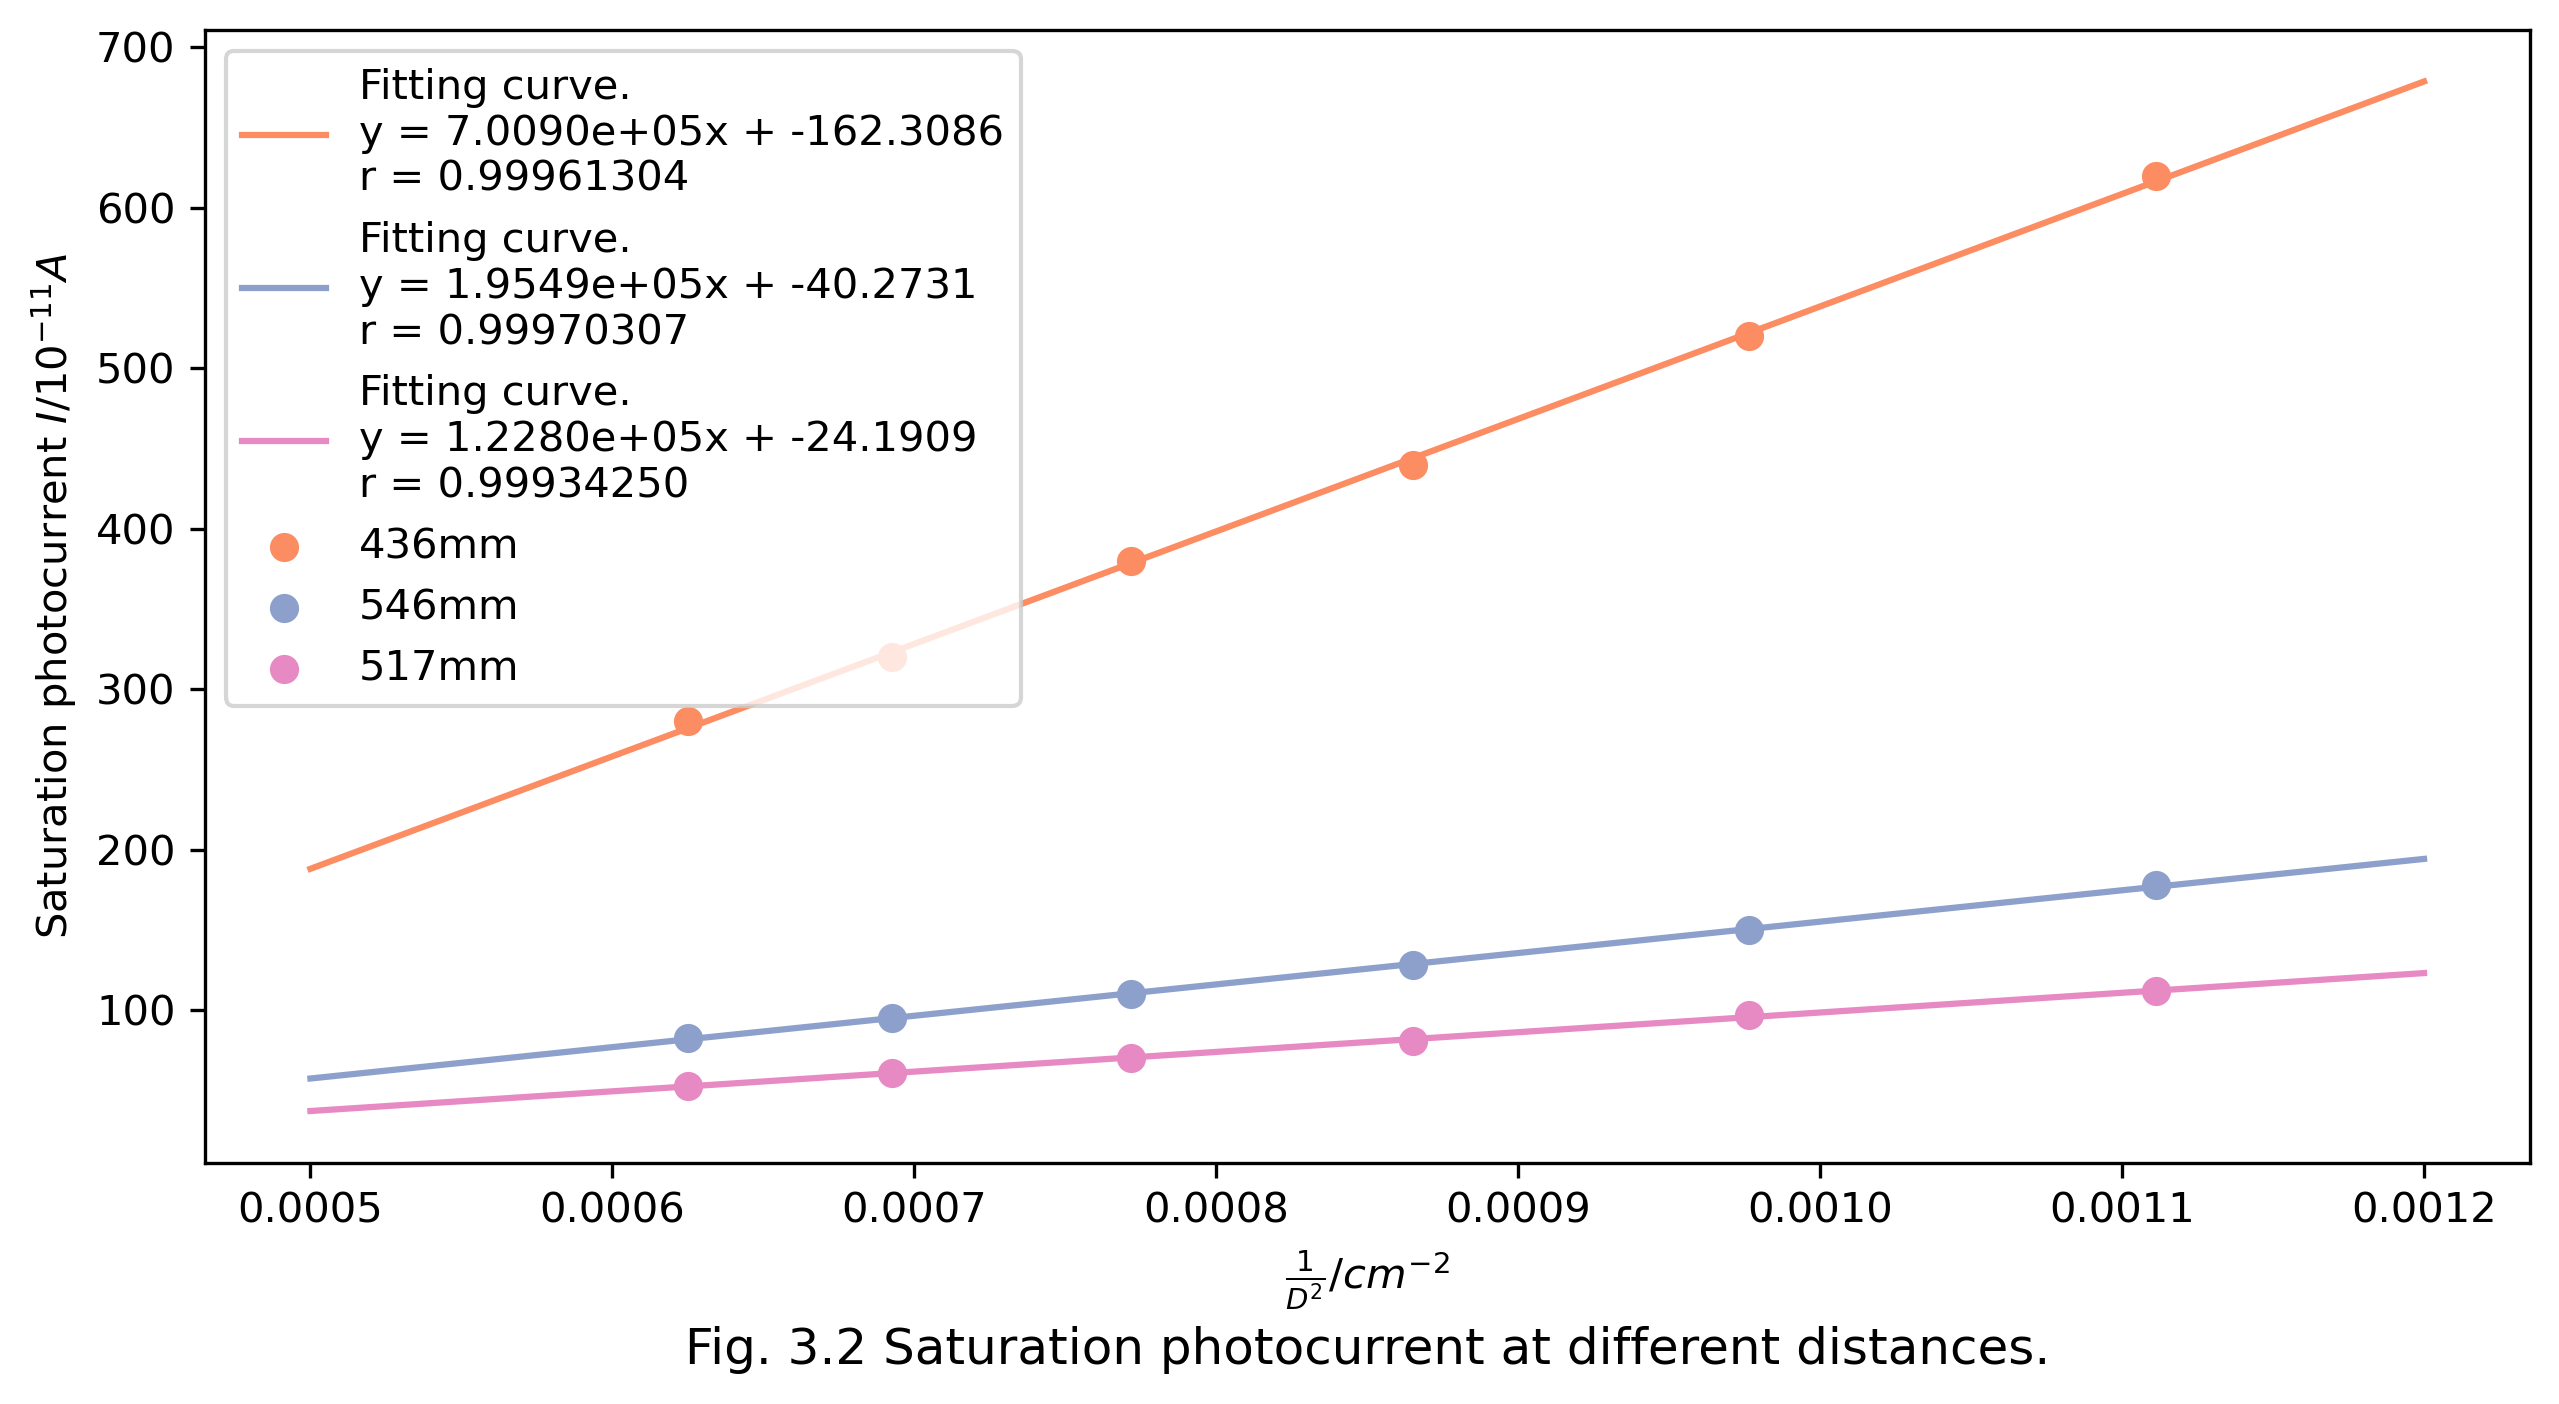
\includegraphics[width=0.7\textwidth]{attachments/fig.3.2.png}
        \caption{饱和光电流和距离平方反比的关系}
        \label{fig:3.2}
    \end{figure}
    实验结果显示饱和光电流和距离平方反比成线性正相关,相关系数$R>0.99$。
    而光强与距离平方反比成正比,因此证明了饱和光电流与入射光强成正比。
    同时随着波长减小,饱和光电流随入射光强增长越快。
\subsection*{【结论和误差分析】}
本实验中,我们使用零电流法测量了普朗克常量,结果为
$h = 6.21 \times 10^{-34} J \cdot s$,实验值与公认值相对误差约$6\%$,测量相对准确。
同时我们研究了伏安特性曲线的基本规律,探究了不同因素(入射光波长,光源距离和光阑口径)对光电效应伏安特性曲线的影响。
最后我们研究了饱和光电流随光强变化,证明了饱和光电流随光强成正比。

实验可能的误差有:
\begin{enumerate}[label=\arabic*.]
    \item 零电流法:由于反向电流的存在,零电流下反向电压并非真正的截止电压
    \item 实验中发现当电压达到$50V$时,光电流仍在以一定速率升高,可能未达到完全饱和。
\end{enumerate}

  
\subsection*{【思考题】}
    \subsubsection*{1. 截止电压的物理意义是什么?}
    逸出的光电子具有一定初动能。当光照射光电管阴极时,光电子逸出而落入阳极形成光电流。
    加上反向电压,使阳极电位降低,直到所有光电子都不能到达阳极,此时光电流为零。
    这个使光电流为零的相对于阴极的反向电压$U_s$称为光电效应的截止电压,有:
    $$
        eU_s = \frac{1}{2}mv^2
    $$
    截止电压是光电子的最大动能全部转化为势能时对应的电压值。
    \subsubsection*{2. 实验仪选择不同的电流灵敏度(即不同的电流测量档)是否会影响普朗克常数的测量?}
    会影响。因为在零电流法测量普朗克常量中,需要准确读出在光电流为零所对应的电压值。
    电流灵敏度越高,电压值越准确,测量精度越高。否则测量普朗克常量误差将比较大。
    \subsubsection*{3. 光电管与光电池有什么区别?}
    光电管是一种光敏电路元件(光电转换器件),受光照后从阴极释放光电子形成光电流,原理是光电效应。
    
    光电池是一种特殊的半导体二极管,利用光伏效应将可见光转化为直流电,从而把光能转换成电能,是电源元件。
    \subsubsection*{4. 本实验最大的误差来源是什么?试提出一些减少实验误差的建议。}
    最大的误差来源是反向电流的存在。由于阳极上往往也溅有少量阴极材料,受光照时也将发射光电子。
    此外,阴极电子也可能被阳极反射。这样,在反向电压的作用下,
    阳极发射的电子受到加速作用而形成反向电流,从而抵消了一部分光电流,给实验带来误差。

    建议:
    \begin{enumerate}[label=\arabic*.]
        \item 增大光源光强,从而增大光电流,掩盖反向电流影响。
        \item 使用新的光电管。
    \end{enumerate}

\subsection*{【项目源码】}
\url{https://github.com/Jeg-Vet/SYSU-PHY-EXP/tree/main/B1-Photoelectric_effect}

\end{document}